\documentclass{article}
\usepackage{mathtools}
\usepackage{color}
\usepackage[utf8]{inputenc}
\usepackage{mathtools}
\usepackage{graphicx}
\usepackage{placeins}
\graphicspath{ {./img/} }
\begin{document}
\title{TDT4136 - Assignment 3}
\author{Filip F Egge}
\date{October 3, 2014}
\maketitle

\newpage
\section*{Problem A - Pathfinding in 2D Games}
\subsection*{Subproblem A.1 - Grids with Obstacles}
	\FloatBarrier
	\begin{figure}[!htb]
		\caption{Board 1-1}
		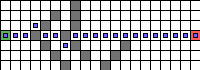
\includegraphics[width=0.9\textwidth]{img1.png}
	\end{figure}

	\begin{figure}[!htb]
		\caption{Board 1-2}
		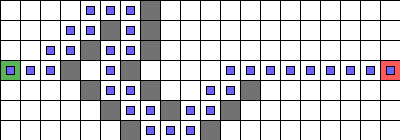
\includegraphics[width=0.9\textwidth]{img2.png}
	\end{figure}
	\begin{figure}[!htb]
		\caption{Board 1-3}
		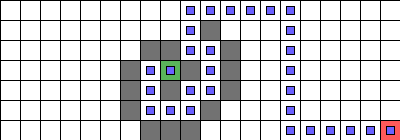
\includegraphics[width=0.9\textwidth]{img3.png}
	\end{figure}
	\begin{figure}[!htb]
		\caption{Board 1-4}
		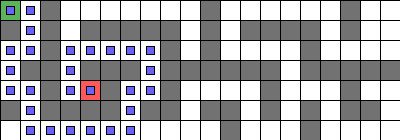
\includegraphics[width=0.9\textwidth]{img4.png}
	\end{figure}
\FloatBarrier
\subsection*{Subproblem A.2 - Grids with Different Cell Costs}
	\begin{figure}[!htb]
		\caption{Board 2-1}
		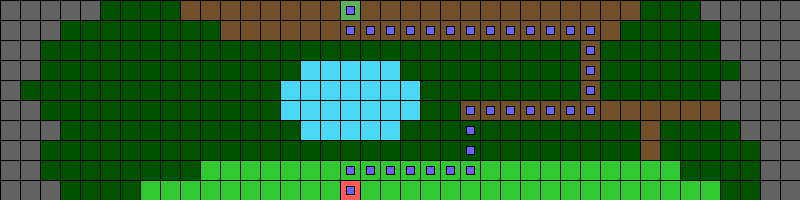
\includegraphics[width=0.9\textwidth]{BImg1.png}
	\end{figure}

	\begin{figure}[!htb]
		\caption{Board 2-2}
		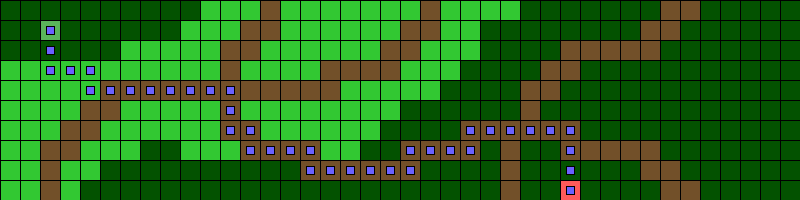
\includegraphics[width=0.9\textwidth]{BImg2.png}
	\end{figure}

	\begin{figure}[!htb]
		\caption{Board 2-3}
		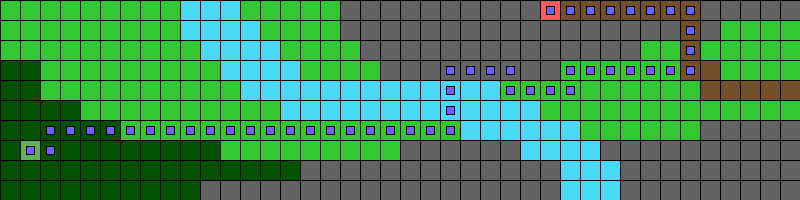
\includegraphics[width=0.9\textwidth]{BImg3.png}
	\end{figure}

	\begin{figure}[!htb]
		\caption{Board 2-4}
		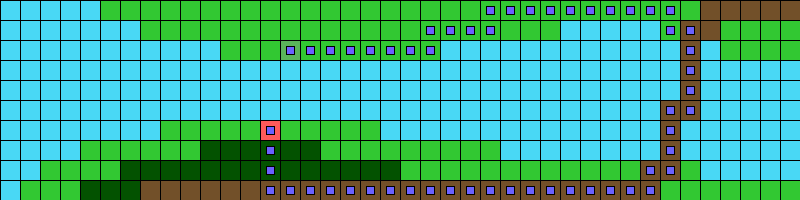
\includegraphics[width=0.9\textwidth]{BImg4.png}
	\end{figure}
\FloatBarrier
\subsection*{Subproblem A.3 Comparison with BFS and Dijkstra's}

	For this part of the exercise i modified BFS to use a FIFO queue and Dijkstra to sort the open list on g(s). This however did not seem to work with my implementation, and i tried finding where i went wrong. I spent to long trying to figure it out, and desided to deliever in it's current state. For the visualization i used red squared for nodes in the closed list, and yellow for nodes in the open list. 

	\begin{figure}[!htb]
		\caption{BFS - Board 1-1}
		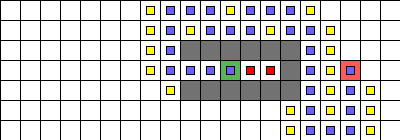
\includegraphics[width=0.9\textwidth]{Bfs1-1.png}
	\end{figure}
	\begin{figure}[!htb]
		\caption{Dijkstra - Board 1-1}
		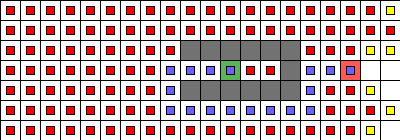
\includegraphics[width=0.9\textwidth]{Dijkstra-1-1.png}
	\end{figure}


	\begin{figure}[!htb]
		\caption{BFS - Board 1-2}
		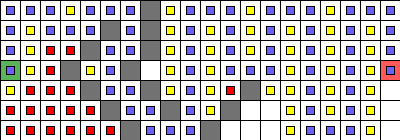
\includegraphics[width=0.9\textwidth]{Bfs1-2.png}
	\end{figure}
	\begin{figure}[!htb]
		\caption{Dijkstra - Board 1-2}
		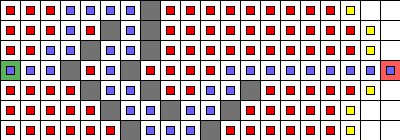
\includegraphics[width=0.9\textwidth]{Dijkstra-1-2.png}
	\end{figure}


	\begin{figure}[!htb]
		\caption{BFS - Board 1-3}
		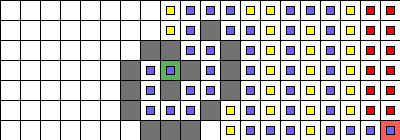
\includegraphics[width=0.9\textwidth]{Bfs1-3.png}
	\end{figure}
	\begin{figure}[!htb]
		\caption{Dijkstra - Board 1-3}
		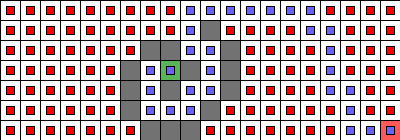
\includegraphics[width=0.9\textwidth]{Dijkstra-1-3.png}
	\end{figure}


	\begin{figure}[!htb]
		\caption{BFS - Board 1-4}
		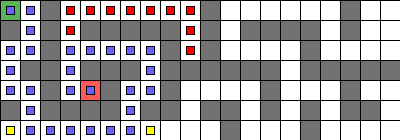
\includegraphics[width=0.9\textwidth]{Bfs1-4.png}
	\end{figure}
	\begin{figure}[!htb]
		\caption{Dijkstra - Board 1-4}
		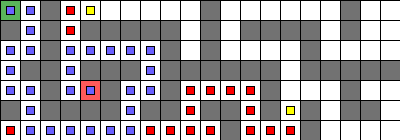
\includegraphics[width=0.9\textwidth]{Dijkstra-1-4.png}
	\end{figure}


	\begin{figure}[!htb]
		\caption{BFS - Board 2-1}
		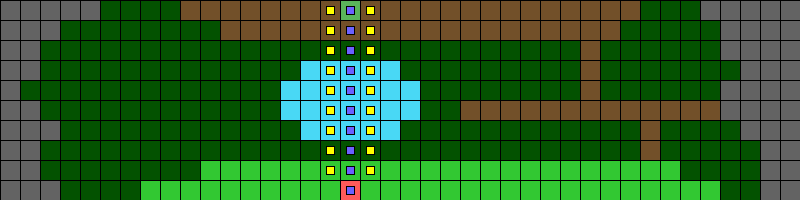
\includegraphics[width=0.9\textwidth]{Bfs2-1.png}
	\end{figure}
	\begin{figure}[!htb]
		\caption{Dijkstra - Board 2-1}
		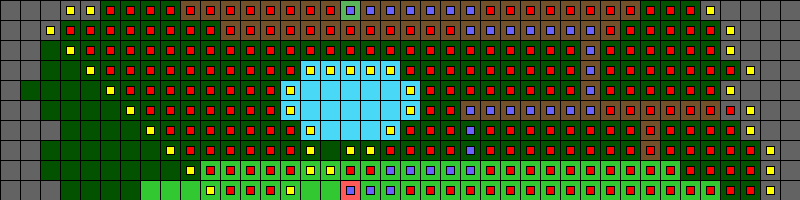
\includegraphics[width=0.9\textwidth]{Dijkstra-2-1.png}
	\end{figure}


	\begin{figure}[!htb]
		\caption{BFS - Board 2-2}
		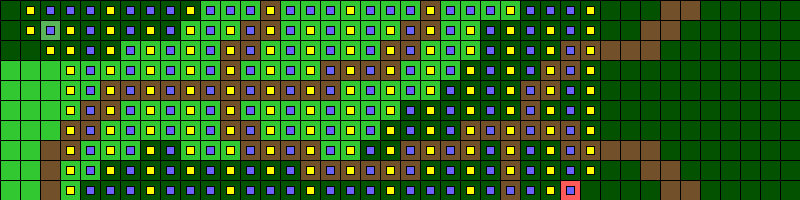
\includegraphics[width=0.9\textwidth]{Bfs2-2.png}
	\end{figure}
	\begin{figure}[!htb]
		\caption{Dijkstra - Board 2-2}
		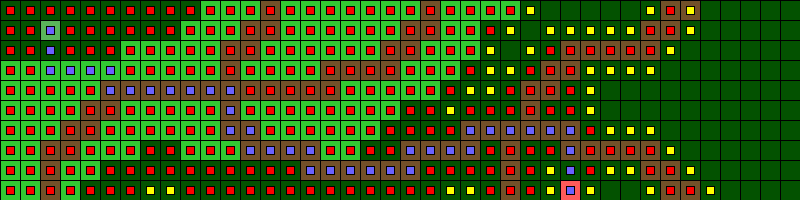
\includegraphics[width=0.9\textwidth]{Dijkstra-2-2.png}
	\end{figure}

	\begin{figure}[!htb]
		\caption{BFS - Board 2-3}
		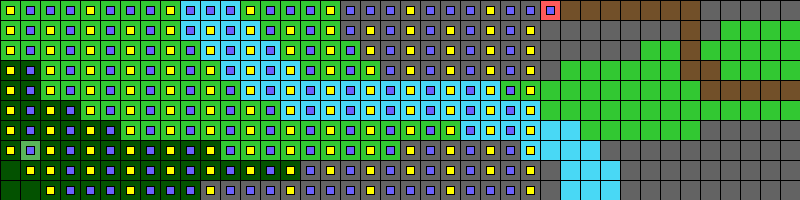
\includegraphics[width=0.9\textwidth]{Bfs2-3.png}
	\end{figure}
	\begin{figure}[!htb]
		\caption{Dijkstra - Board 2-3}
		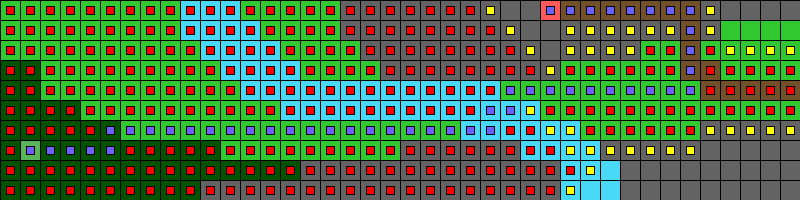
\includegraphics[width=0.9\textwidth]{Dijkstra-2-3.png}
	\end{figure}

	\begin{figure}[!htb]
		\caption{BFS - Board 2-4}
		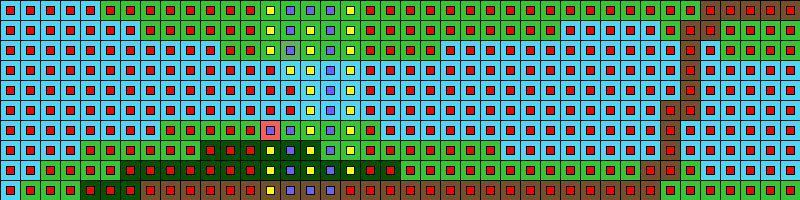
\includegraphics[width=0.9\textwidth]{Bfs2-4.png}
	\end{figure}
	\begin{figure}[!htb]
		\caption{Dijkstra - Board 2-4}
		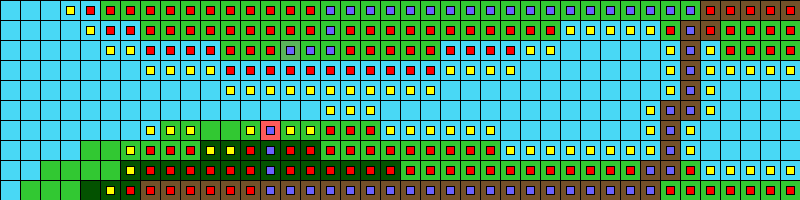
\includegraphics[width=0.9\textwidth]{Dijkstra-2-4.png}
	\end{figure}
\end{document}